\chapter{Equity Derivatives Beyond Vanilla}
\label{ch:equity_derivatives}
\chaptermark{Equity derivatives beyond vanilla}

\Cref{ch:black_scholes} gave Black--Scholes; \cref{ch:vol_surface} showed
the market violates its flat-vol assumption, producing a surface. This
chapter covers three progressively richer models of that surface:
\emph{local volatility} (Dupire), \emph{stochastic volatility} (Heston),
and their combination \emph{local-stochastic volatility} (LSV). It then
derives the variance swap. The variance-swap replication formula,
promised in \cref{ch:vol_surface}, is the centrepiece: it ties together
the vol surface, the $1/\Kstrike^2$ option-strip hedge, and the desk
workflow for trading pure volatility.

\begin{backgroundbox}[Prerequisites]
From earlier in the book:
\begin{itemize}
  \item \Cref{ch:black_scholes}: Black--Scholes PDE and formula,
    risk-neutral pricing under GBM, the assumptions (constant
    $\volat$, continuous hedging, no dividends).
  \item \Cref{ch:greeks_hedging}: delta, gamma, vega, theta; the
    delta-hedged P\&L identity $d\Pi \approx \tfrac12\,\Gamma\,\Spx^2\,
    (\volat_{\text{r}}^2 - \volat_{\text{i}}^2)\,dt$; long gamma
    profits when realised vol exceeds implied.
  \item \Cref{ch:vol_surface}: implied vol, smile/skew, variance-swap
    definition (\cref{def:varswap}), and the schematic replication
    (\cref{eq:varswap_replication}) whose derivation we give here.
\end{itemize}
Re-read those chapters if hazy.
\end{backgroundbox}


%% ================================================================
\section{Local volatility (Dupire)}
\label{sec:local_vol}
%% ================================================================

Black--Scholes assumes constant $\volat$. The simplest generalisation
lets volatility depend on the underlying's level and on time:
\begin{equation}
  d\Spx_t \;=\; \rrf\,\Spx_t\,dt
              \;+\; \volat_{\text{loc}}(\Spx_t, t)\,\Spx_t\,dW_t,
  \label{eq:local_vol_sde}
\end{equation}
where $\volat_{\text{loc}}(\Spx, t)$ is the \textbf{local volatility
function}, a deterministic surface that can in principle be chosen
so the model reproduces every observed European-option price
simultaneously. Because $\volat_{\text{loc}}$ is a known function of
$(\Spx, t)$, the model is Markovian and the Kolmogorov forward
equation pins down the risk-neutral density at every maturity.

\subsection{Dupire's formula}
\label{subsec:dupire_formula}

\citet{dupire1994pricing} and \citet{derman1994riding} independently
found an explicit expression for $\volat_{\text{loc}}^2$ in terms of
the market call surface $\Call(\Kstrike, \Tmat)$:

\begin{keyfactbox}[Dupire's local volatility formula]
\label{fact:dupire}
If European call prices $\Call(\Kstrike,\Tmat)$ are known for all
strikes $\Kstrike > 0$ and maturities $\Tmat > 0$, the unique
diffusion coefficient that reproduces those prices is
\begin{equation}
  \volat_{\text{loc}}^2(\Kstrike,\Tmat)
  \;=\;
  \frac{\dfrac{\partial \Call}{\partial \Tmat}
        \;+\; \rrf\,\Kstrike\,\dfrac{\partial \Call}{\partial \Kstrike}}
       {\dfrac{1}{2}\,\Kstrike^2\,
        \dfrac{\partial^2 \Call}{\partial \Kstrike^2}}.
  \label{eq:dupire}
\end{equation}
\end{keyfactbox}

\noindent
\textbf{Reading the formula.}
\begin{itemize}
  \item The \emph{numerator} measures how the call price changes with
    maturity (plus a drift correction); the rate at which value
    accrues with $\Tmat$ encodes the local variance needed at $(K,T)$.
  \item The \emph{denominator} is $\tfrac12 K^2$ times the butterfly
    spread. By Breeden--Litzenberger, $\partial^2\Call/\partial
    \Kstrike^2 = e^{-\rrf\Tmat}p(\Kstrike,\Tmat)$, so the denominator
    normalises by the risk-neutral probability of landing near
    $\Kstrike$.
  \item The ratio answers: given where the market thinks
    $\Spx_\Tmat$ can be, how much diffusion does the model need at
    that point?
\end{itemize}

\noindent
\textbf{In practice.} Dupire is applied not to raw prices but to a
smooth parametric fit of the implied-vol surface (SVI/SABR from
\cref{ch:vol_surface}); partial derivatives are computed analytically
from the fit, avoiding the noise of finite-differencing sparse quotes.

\subsection{Local vol in practice: from the surface to a function}
\label{subsec:local_vol_practice}

The desk workflow for local-vol calibration:
\begin{enumerate}
  \item \textbf{Fit a smooth implied-vol surface} (SVI, SABR, or a
    spline) to market quotes, giving continuous
    $\volat_{\text{imp}}(\Kstrike, \Tmat)$.
  \item \textbf{Convert to call prices} via Black--Scholes.
  \item \textbf{Apply Dupire's formula.} Compute the three partials
    in \cref{eq:dupire} analytically or by finite differences to
    evaluate $\volat_{\text{loc}}^2$ on a grid.
  \item \textbf{Interpolate} the grid for pricing.
\end{enumerate}

\noindent
\textbf{Qualitative example.} A 3-month surface with 25-delta put vol
25\%, ATM 20\%, 25-delta call 17\% yields a Dupire local-vol function
higher at low spot ($\approx 28\%$ at $\Spx=3{,}600$) and lower at
high spot ($\approx 15\%$ at $\Spx=4{,}400$): the skew is ``explained''
by assigning more diffusion where the market prices fat tails.

\begin{keyfactbox}[Local vol vs implied vol]
Local and implied vol are distinct quantities (both depend on
$(K,T)$). Implied vol is the constant $\volat$ that reproduces a
single option price via Black--Scholes; local vol is the
\emph{instantaneous} diffusion coefficient at $(\Spx,t)$ in a model
reproducing \emph{all} prices. Roughly, implied vol is a
path-weighted average of local vol from $\Spx_0$ to $\Kstrike$. A
\citet{dupire1994pricing} rule of thumb: local vol $\approx$ twice
implied vol minus the ATM level (near-ATM, first order).
\end{keyfactbox}

\begin{pitfallbox}[Local vol is static]
\label{pitfall:local_vol_static}
Local vol fits today's surface exactly by construction but assumes
$\volat_{\text{loc}}(\Spx,t)$ is deterministic and fixed at time 0.
Tomorrow's surface will differ, and the model has no mechanism for
the change: it predicts skew flattens with maturity far faster than
markets actually exhibit. Traders say local vol gets statics right
but dynamics wrong. Delta-hedging exotics with local-vol Greeks
leaves you systematically mis-hedged when the smile shifts; hence
Heston and LSV.
\end{pitfallbox}

\begin{intuitionbox}
Local vol is a \emph{photograph} of today's surface: pixel-perfect
but frozen. Heston is a \emph{physical model}: may miss wrinkles
but has built-in dynamics (mean-reversion, vol-of-vol, spot--vol
correlation) that produce plausible future surfaces. LSV combines
both: photo today, physics tomorrow.
\end{intuitionbox}


%% ================================================================
\section{Heston stochastic volatility}
\label{sec:heston}
%% ================================================================

Local vol makes volatility a deterministic function of spot and time.
Heston~\citep{heston1993closed} takes the opposite approach: volatility
is itself a random process, correlated with the spot.

\subsection{The Heston SDE}
\label{subsec:heston_sde}

Under the risk-neutral measure, the Heston dynamics are:
\begin{align}
  d\Spx_t &= \rrf\,\Spx_t\,dt
              + \sqrt{v_t}\,\Spx_t\,dW_1(t),
  \label{eq:heston_spot} \\
  dv_t    &= \kappa\,(\bar{v} - v_t)\,dt
              + \xi\,\sqrt{v_t}\,dW_2(t),
  \label{eq:heston_var} \\
  \rho    &= \Corr(dW_1, dW_2),
  \notag
\end{align}
where $v_t = \volat_t^2$ is the instantaneous variance (not
volatility), and the five parameters are:

\begin{keyfactbox}[Heston model parameters]
\label{fact:heston_params}
\begin{center}
\begin{tabular}{cll}
  \toprule
  Symbol & Name & Typical equity value \\
  \midrule
  $\kappa$ & Mean-reversion speed of variance
           & $1$--$5\;\text{yr}^{-1}$ \\
  $\bar{v}$ & Long-run variance ($= \bar\sigma^2$)
             & $(0.20)^2 = 0.04$ \\
  $\xi$     & Vol of vol (volatility of $v_t$)
             & $0.3$--$1.0$ \\
  $\rho$    & Spot--vol correlation
             & $-0.9$ to $-0.5$ \\
  $v_0$     & Initial variance ($= \sigma_0^2$)
             & Calibrated to ATM vol \\
  \bottomrule
\end{tabular}
\end{center}
\end{keyfactbox}

\noindent
\textbf{Reading the SDE.}
\begin{itemize}
  \item \emph{Variance mean-reverts.} \Cref{eq:heston_var} is a
    Cox--Ingersoll--Ross (CIR) process: when $v_t > \bar v$ the drift
    pulls down, and vice versa, at speed $\kappa$. The
    \textbf{Feller condition} $2\kappa\bar v \geq \xi^2$ keeps $v_t$
    strictly positive.
  \item \emph{Spot inherits stochastic vol.} \Cref{eq:heston_spot}
    is GBM with $\sqrt{v_t}$ replacing constant $\volat$.
  \item \emph{$\rho$ creates skew.} Negative $\rho$ (typical for
    equities) means falling spot coincides with rising variance,
    fattening the left tail and making OTM puts expensive.
\end{itemize}

\begin{intuitionbox}[title={Why negative $\rho$ creates skew}]
\label{intuition:heston_rho}
Market drops coincide with vol spikes: the \emph{leverage effect}.
Heston bakes this in: $\rho<0$ correlates negative spot returns with
positive variance shocks, producing a fat left tail (i.e.\ higher
implied vol at low strikes). More negative $\rho$, steeper skew;
$\rho=0$ yields a symmetric smile rarely seen in equities.
\end{intuitionbox}

\subsection{Characteristic-function pricing}
\label{subsec:heston_cf}

Heston's key contribution: despite the 2D SDE, European calls admit a
semi-closed-form price via the characteristic function of $\ln\Spx_\Tmat$.

Because the Heston SDE is \emph{affine} (drift and diffusion of
log-spot and variance are affine in the state), the characteristic
function $\varphi(u)=\E^{\Qm}[e^{iu\ln\Spx_\Tmat}]$ solves Riccati
ODEs with closed-form solutions. The call price is
\begin{equation}
  \Call(\Kstrike, \Tmat)
  \;=\;
  \Spx_0\,\Pi_1 \;-\; \Kstrike\,e^{-\rrf \Tmat}\,\Pi_2,
  \label{eq:heston_call}
\end{equation}
where
\begin{equation}
  \Pi_j
  \;=\;
  \frac{1}{2}
  \;+\;
  \frac{1}{\pi}\int_0^{\infty}
    \operatorname{Re}\!\left[
      \frac{e^{-iu\ln \Kstrike}\,\varphi_j(u)}{iu}
    \right] du,
  \qquad j = 1, 2.
  \label{eq:heston_pi}
\end{equation}
$\varphi_1,\varphi_2$ are closed-form (complex exponentials of the
parameters), and the 1D integrals in \eqref{eq:heston_pi} need only a
few dozen quadrature points for six-digit accuracy, fast enough for
real-time calibration.

\begin{keyfactbox}[Heston pricing is semi-closed-form]
The characteristic-function approach needs one 1D integral, orders
of magnitude faster than Monte Carlo, enabling sub-second calibration
to the full surface. The same structure extends to other affine
stochastic-vol models (Bates, double Heston).
\end{keyfactbox}

\subsection{How each parameter shapes the smile}
\label{subsec:heston_params_smile}

Varying each parameter from a baseline $v_0=\bar v=0.04$
($\sigma=20\%$), $\kappa=2$, $\xi=0.5$, $\rho=-0.7$:

\begin{center}
\begin{tabular}{lp{8cm}}
  \toprule
  Parameter change & Effect on implied-vol smile \\
  \midrule
  $\rho$: $-0.7 \to -0.3$ &
    Skew decreases.  The smile becomes more symmetric: less steep
    on the left, slightly higher on the right.  The left-tail fattening
    diminishes because spot and vol are less anti-correlated. \\[6pt]
  $\xi$: $0.5 \to 1.0$ &
    Both wings rise.  The smile becomes more curved (higher curvature
    = fatter tails on both sides).  Vol of vol injects randomness into
    the variance process, creating a wider distribution for
    $\Spx_\Tmat$. \\[6pt]
  $\kappa$: $2 \to 5$ &
    Smile \emph{flattens at long maturities}.  Strong mean-reversion
    pulls $v_t$ back to $\bar{v}$ quickly, so the long-dated
    distribution looks more Gaussian (less smile).  Short-dated
    smiles are less affected. \\[6pt]
  $v_0$: $0.04 \to 0.09$ ($\sigma_0 = 30\%$) &
    The entire smile shifts upward.  The level of ATM vol rises.
    The shape (skew, curvature) is largely unchanged because those
    are controlled by $\rho$ and $\xi$. \\
  \bottomrule
\end{tabular}
\end{center}

\begin{figure}[htbp]
\centering
\begin{minipage}{0.48\textwidth}
\centering
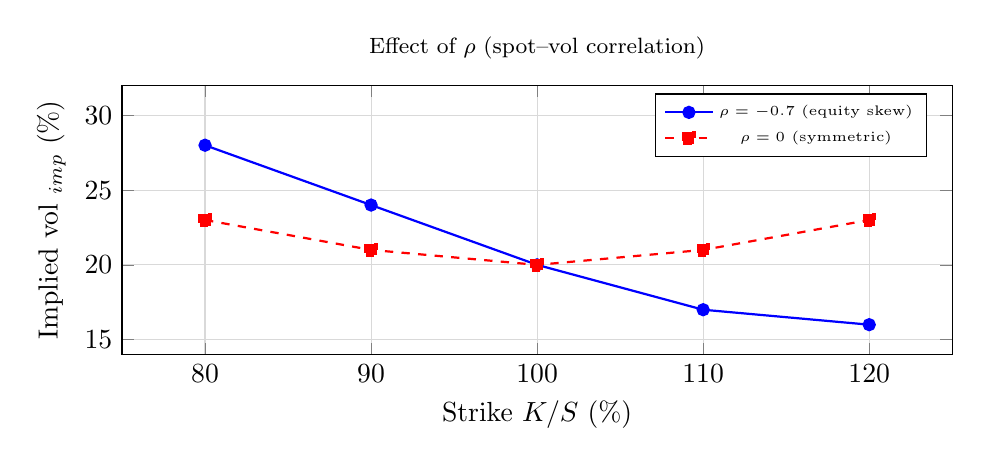
\begin{tikzpicture}
\begin{axis}[
  width=\textwidth, height=5cm,
  xlabel={Strike $K/S$ (\%)},
  ylabel={Implied vol $\volat_{\text{imp}}$ (\%)},
  xmin=75, xmax=125,
  ymin=14, ymax=32,
  xtick={80,90,100,110,120},
  legend style={at={(0.97,0.97)}, anchor=north east, font=\tiny},
  grid=major, grid style={gray!30},
  title={\footnotesize Effect of $\rho$ (spot--vol correlation)},
]
\addplot[blue, thick, mark=*] coordinates {
  (80,28)(90,24)(100,20)(110,17)(120,16)};
\addlegendentry{$\rho=-0.7$ (equity skew)}
\addplot[red, thick, dashed, mark=square*] coordinates {
  (80,23)(90,21)(100,20)(110,21)(120,23)};
\addlegendentry{$\rho=0$ (symmetric)}
\end{axis}
\end{tikzpicture}
\end{minipage}
\hfill
\begin{minipage}{0.48\textwidth}
\centering
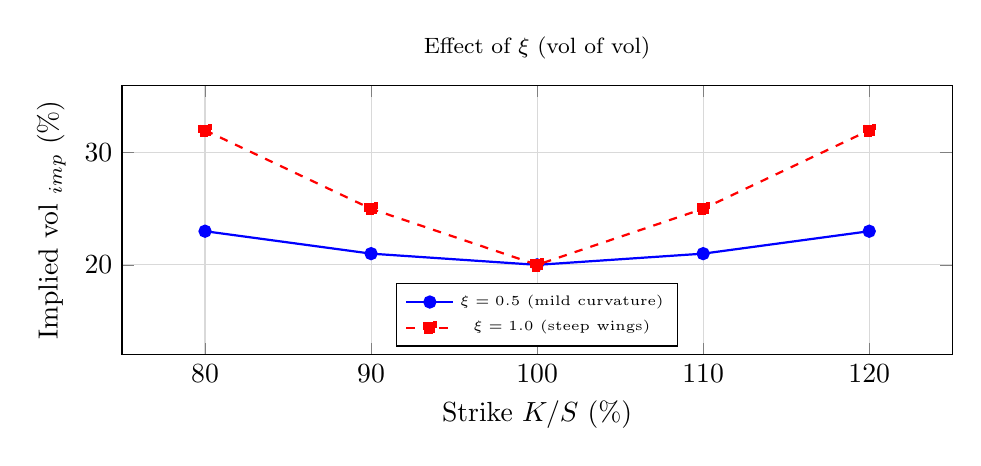
\begin{tikzpicture}
\begin{axis}[
  width=\textwidth, height=5cm,
  xlabel={Strike $K/S$ (\%)},
  ylabel={Implied vol $\volat_{\text{imp}}$ (\%)},
  xmin=75, xmax=125,
  ymin=12, ymax=36,
  xtick={80,90,100,110,120},
  legend style={at={(0.5,0.03)}, anchor=south, font=\tiny},
  grid=major, grid style={gray!30},
  title={\footnotesize Effect of $\xi$ (vol of vol)},
]
\addplot[blue, thick, mark=*] coordinates {
  (80,23)(90,21)(100,20)(110,21)(120,23)};
\addlegendentry{$\xi=0.5$ (mild curvature)}
\addplot[red, thick, dashed, mark=square*] coordinates {
  (80,32)(90,25)(100,20)(110,25)(120,32)};
\addlegendentry{$\xi=1.0$ (steep wings)}
\end{axis}
\end{tikzpicture}
\end{minipage}
\caption{Heston smile sensitivities from baseline $v_0=\bar{v}=0.04$ ($\volat=20\%$),
$\kappa=2$. \textbf{Left:} negative $\rho$ tilts the smile into an equity skew: OTM puts
expensive, OTM calls cheap. \textbf{Right:} higher $\xi$ lifts both wings symmetrically,
producing curvature without skew.}
\label{fig:heston_smile}
\end{figure}

\noindent
Worth memorising: calibrate $v_0$ to ATM vol, $\rho$ to 25-delta risk
reversal (skew), $\xi$ to 25-delta butterfly (curvature), $\kappa$ to
the smile's term structure. $\bar v$ is often pinned to $v_0$ for
short dates and only matters at long maturities.

\subsection{Calibration workflow}
\label{subsec:heston_calib}

Heston calibration minimises the distance between model and market
implied vols over the five parameters:
\begin{equation}
  \min_{v_0, \kappa, \bar{v}, \xi, \rho}\;
  \sum_{i=1}^{N}
    w_i\,\bigl[
      \volat_{\text{Heston}}(\Kstrike_i, \Tmat_i;\, v_0, \kappa, \bar{v}, \xi, \rho)
      \;-\;
      \volat_{\text{mkt}}(\Kstrike_i, \Tmat_i)
    \bigr]^2,
  \label{eq:heston_calib}
\end{equation}
with $w_i$ vega- or uniform-weighted and $\volat_{\text{Heston}}$ the
model implied vol (from \cref{eq:heston_call}, then inverting BS).

The objective is non-convex, so global optimisers (differential
evolution, simulated annealing) beat gradient methods. For $N=50$
quotes, total cost is $\sim 12{,}500$ characteristic-function
evaluations, sub-second on modern hardware.

\begin{pitfallbox}[Feller condition and calibration]
An optimiser may propose parameters violating $2\kappa\bar v\geq\xi^2$,
letting $v_t$ touch zero and breaking the characteristic function.
``Full truncation'' schemes tolerate this but produce degenerate
paths; safer to impose Feller as a calibration constraint.
\end{pitfallbox}

\subsection{What Heston gets right and wrong}
\label{subsec:heston_tradeoffs}

Heston's five parameters capture the qualitative equity-surface shape
($\rho$ skew, $\xi$ curvature, $\bar v, v_0$ level, $\kappa$ term
structure) but cannot exactly match every kink. Failure modes:

\begin{itemize}
  \item \textbf{Short-dated smile.} Continuous CIR variance misses
    the vol jumps that steepen short wings in real markets.
  \item \textbf{Wings.} Heston's asymptotics as $\Kstrike\to 0,\infty$
    may not match the market's.
  \item \textbf{Across maturities.} Constant parameters force a
    specific short-vs-long smile relationship; real surfaces violate
    it, requiring piecewise-constant calibration.
\end{itemize}

\noindent
Desks use piecewise-constant parameters across maturity buckets, add
jumps (the Bates model: spot + Poisson jumps), or combine Heston with
local vol, the subject of the next section.

\subsection{Comparison: Black--Scholes vs local vol vs Heston}
\label{subsec:model_comparison}

\begin{center}
\begin{tabular}{lccc}
  \toprule
  Feature & Black--Scholes & Local vol & Heston \\
  \midrule
  Vol assumption & Constant $\volat$ & $\volat(\Spx,t)$ deterministic
    & $v_t$ stochastic \\
  Fits today's surface? & No (flat) & Yes (exactly) & Approximately \\
  Smile dynamics? & None & Wrong (too flat) & Realistic \\
  Free parameters & 1 ($\volat$) & $\infty$ (the function) & 5 \\
  Pricing speed & Closed-form & PDE/MC & Semi-closed-form \\
  Use case & Pedagogy, quotes & Vanilla Greeks & Exotic pricing \\
  \bottomrule
\end{tabular}
\end{center}


%% ================================================================
\section{Local-stochastic volatility (LSV)}
\label{sec:lsv}
%% ================================================================

LSV combines both approaches:
\begin{equation}
  d\Spx_t
  \;=\;
  \rrf\,\Spx_t\,dt
  \;+\;
  L(\Spx_t, t)\,\sqrt{v_t}\,\Spx_t\,dW_1(t),
  \label{eq:lsv_sde}
\end{equation}
where $v_t$ follows Heston dynamics and $L(\Spx,t)$ is a
\textbf{leverage function} calibrated so the model reproduces today's
surface exactly. The stochastic part $\sqrt{v_t}$ supplies realistic
dynamics; the local part $L$ bends prices to match every quote.

\begin{keyfactbox}[LSV is the industry standard]
LSV is the standard for pricing and hedging exotic equity
derivatives: Heston-like dynamics for exotics whose value depends on
the future smile (barriers, cliquets, autocallables), and exact
vanilla calibration. Calibrating $L(\Spx,t)$ (particle methods or
forward PDE) is expensive but gives the most internally consistent
framework available.
\end{keyfactbox}

\noindent
\textbf{The leverage function.} With Dupire local vol
$\volat_{\text{loc}}(\Spx,t)$,
\begin{equation}
  L(\Spx,t)
  \;=\;
  \frac{\volat_{\text{loc}}(\Spx,t)}
       {\sqrt{\E[v_t \mid \Spx_t = \Spx]}},
  \label{eq:leverage_function}
\end{equation}
where the conditional expectation is under the model's own joint
$(\Spx_t,v_t)$ distribution. This fixed-point equation forces
iterative calibration (particle MC or Fokker--Planck PDE).

\noindent
\textbf{Mixing-fraction intuition.} Parametrise by $\alpha\in[0,1]$:
\begin{itemize}
  \item $\alpha=0$: pure local vol (perfect fit, wrong dynamics).
  \item $\alpha=1$: pure Heston (right dynamics, imperfect fit).
  \item $\alpha\in(0,1)$: LSV, where $L$ bends Heston to fit exactly
    while retaining fraction $\alpha$ of the stochastic dynamics.
\end{itemize}
$\alpha$ is set to match observed surface dynamics (e.g.\ skew shift
per 1\% spot move); equity desks typically use $\alpha\approx0.5$--$0.8$.


%% ================================================================
\section{Variance swap replication}
\label{sec:varswap_replication}
%% ================================================================

This section delivers the derivation promised in
\cref{ch:vol_surface}: the fair variance-swap strike equals a
$1/\Kstrike^2$-weighted integral of OTM option prices. The argument
is model-independent (it holds for any continuous diffusion, not just
BS or Heston) and is one of the most elegant results in quant finance.

\emph{Why the product exists.} An option gives vol exposure, but only
bundled with directional exposure that must be neutralised by daily
delta-hedging; the realised P\&L depends on the hedging path
(\cref{ch:greeks_hedging}). A variance swap pays realised variance
directly, so a trader who wants a pure view on volatility can buy one
and skip the hedging workflow entirely; the dealer handles replication.

\subsection{Setup and payoff}
\label{subsec:varswap_setup}

Recall the variance-swap definition from \cref{def:varswap}.  The
buyer receives at maturity $\Tmat$:
\[
  \text{Payoff}
  \;=\;
  N \,\bigl(\,\volat_{\text{r}}^2 \;-\; \Kstrike_{\text{var}}\,\bigr),
\]
where $\volat_{\text{r}}^2$ is the annualised realised variance of
$\ln \Spx$ over $[0,\Tmat]$ and $\Kstrike_{\text{var}}$ is the
\emph{variance strike} (here expressed in variance units, not vol
units).  The fair strike $\Kstrike_{\text{var}}$ is the value that
makes the swap worth zero at inception:
\begin{equation}
  \Kstrike_{\text{var}}
  \;=\;
  \E^{\Qm}\!\bigl[\,\volat_{\text{r}}^2\,\bigr].
  \label{eq:varswap_fair_strike}
\end{equation}
Our goal is to express this expectation in terms of observable European
option prices.

\subsection{The log contract}
\label{subsec:log_contract}

A \textbf{log contract} pays $\ln(\Spx_\Tmat/F_0)$ at $\Tmat$, where
$F_0=\Spx_0\,e^{\rrf\Tmat}$. Its risk-neutral expectation ties directly
to realised variance:

\begin{lemma}[Log contract and realised variance]
\label{lem:log_contract}
Under any continuous-path diffusion
$d\Spx_t = \rrf\,\Spx_t\,dt + \volat(t)\,\Spx_t\,dW_t$
(with $\volat(t)$ possibly random), we have
\begin{equation}
  \E^{\Qm}\!\!\left[\ln\frac{\Spx_\Tmat}{F_0}\right]
  \;=\;
  -\,\frac{1}{2}\,\E^{\Qm}\!\!\left[
    \int_0^{\Tmat}\!\volat^2(t)\,dt
  \right]
  \;=\;
  -\,\frac{\Tmat}{2}\,\Kstrike_{\text{var}}.
  \label{eq:log_contract_expectation}
\end{equation}
\end{lemma}

\begin{proof}
Apply It\^o's lemma to $\ln \Spx_t$:
\[
  d\ln \Spx_t
  \;=\;
  \frac{1}{\Spx_t}\,d\Spx_t
  \;-\;
  \frac{1}{2\,\Spx_t^2}\,(d\Spx_t)^2
  \;=\;
  \left(\rrf - \tfrac{1}{2}\volat^2(t)\right)dt
  \;+\;
  \volat(t)\,dW_t.
\]
Integrate from $0$ to $\Tmat$:
\[
  \ln \Spx_\Tmat - \ln \Spx_0
  \;=\;
  \rrf\,\Tmat
  \;-\;
  \frac{1}{2}\int_0^{\Tmat}\!\volat^2(t)\,dt
  \;+\;
  \int_0^{\Tmat}\!\volat(t)\,dW_t.
\]
Since $F_0 = \Spx_0\,e^{\rrf\Tmat}$, we have
$\ln(\Spx_\Tmat / F_0) = \ln \Spx_\Tmat - \ln \Spx_0 - \rrf\Tmat$,
so
\[
  \ln\frac{\Spx_\Tmat}{F_0}
  \;=\;
  -\,\frac{1}{2}\int_0^{\Tmat}\!\volat^2(t)\,dt
  \;+\;
  \underbrace{\int_0^{\Tmat}\!\volat(t)\,dW_t}_{\text{mean-zero martingale}}.
\]
Taking risk-neutral expectations, the It\^o integral vanishes (it is a
mean-zero martingale), giving
\[
  \E^{\Qm}\!\!\left[\ln\frac{\Spx_\Tmat}{F_0}\right]
  \;=\;
  -\,\frac{1}{2}\,\E^{\Qm}\!\!\left[
    \int_0^{\Tmat}\!\volat^2(t)\,dt
  \right]
  \;=\;
  -\,\frac{\Tmat}{2}\,\Kstrike_{\text{var}}.
  \qedhere
\]
\end{proof}

\noindent
Rearranging:
\begin{equation}
  \Kstrike_{\text{var}}
  \;=\;
  -\,\frac{2}{\Tmat}\,
  \E^{\Qm}\!\!\left[\ln\frac{\Spx_\Tmat}{F_0}\right]
  \;=\;
  \frac{2}{\Tmat}\,
  \E^{\Qm}\!\!\left[\ln\frac{F_0}{\Spx_\Tmat}\right].
  \label{eq:kvar_from_log}
\end{equation}
The problem reduces to pricing the log contract
$-\ln(\Spx_\Tmat / F_0)$.

\subsection{Replicating the log payoff with options}
\label{subsec:log_replication}

The key step expresses $-\ln(\Spx_\Tmat/F_0)$ as a static portfolio
of European puts and calls, via an integration-by-parts identity.

\begin{proposition}[Carr--Madan decomposition of a convex payoff]
\label{prop:carr_madan}
For any twice-differentiable function $g:\mathbb{R}_{>0}\to\mathbb{R}$
and any reference level $\kappa > 0$,
\begin{equation}
  g(\Spx_\Tmat)
  \;=\;
  g(\kappa)
  \;+\;
  g'(\kappa)\,(\Spx_\Tmat - \kappa)
  \;+\;
  \int_0^{\kappa} g''(K)\,(K - \Spx_\Tmat)^+\,dK
  \;+\;
  \int_{\kappa}^{\infty} g''(K)\,(\Spx_\Tmat - K)^+\,dK.
  \label{eq:carr_madan}
\end{equation}
\end{proposition}

Any smooth payoff decomposes into a constant, a forward, and a
continuum of puts ($K<\kappa$) and calls ($K>\kappa$) weighted by
$g''(K)$.

\begin{proof}[Proof of \cref{prop:carr_madan}]
Fix $x=\Spx_\Tmat>0$ and $\kappa>0$. Taylor with integral remainder:
\[
  g(x) = g(\kappa) + g'(\kappa)(x - \kappa)
  + \int_\kappa^x g''(u)\,(x - u)\,du.
\]
Split into two cases. For $x>\kappa$:
\[
  \int_\kappa^x g''(u)(x - u)\,du
  = \int_\kappa^\infty g''(K)\,(x - K)^+\,dK,
\]
since $(x-K)^+=x-K$ for $K\leq x$ and 0 otherwise. For $x<\kappa$,
$-\int_x^\kappa g''(u)(u-x)\,du$ equals
\[
  \int_0^\kappa g''(K)\,(K - x)^+\,dK.
\]
Summing covers all cases and gives \cref{eq:carr_madan}.
\end{proof}

\medskip
\noindent
\textbf{Apply to $g(x)=-\ln(x/F_0)$ with $\kappa=F_0$:}
\begin{align*}
  g(F_0) &= -\ln(F_0/F_0) = 0, \\
  g'(x)  &= -\frac{1}{x}, \quad\text{so}\quad
             g'(F_0) = -\frac{1}{F_0}, \\
  g''(x) &= \frac{1}{x^2}.
\end{align*}
Substituting into \cref{eq:carr_madan}:
\begin{equation}
  -\ln\frac{\Spx_\Tmat}{F_0}
  \;=\;
  \underbrace{-\frac{1}{F_0}\,(\Spx_\Tmat - F_0)}_{\text{short
    $1/F_0$ forwards}}
  \;+\;
  \underbrace{\int_0^{F_0}
    \frac{1}{K^2}\,(K - \Spx_\Tmat)^+\,dK}_{\text{OTM puts}}
  \;+\;
  \underbrace{\int_{F_0}^{\infty}
    \frac{1}{K^2}\,(\Spx_\Tmat - K)^+\,dK}_{\text{OTM calls}}.
  \label{eq:log_payoff_decomposition}
\end{equation}

\subsection{From the log contract to the variance-swap strike}
\label{subsec:varswap_formula}

Take risk-neutral expectations of \cref{eq:log_payoff_decomposition}
and price at time 0 (payoff $X$ at $\Tmat$ costs
$e^{-\rrf\Tmat}\E^{\Qm}[X]$):
\begin{itemize}
  \item Log-contract price: $e^{-\rrf\Tmat}\E^{\Qm}[-\ln(\Spx_\Tmat/F_0)]$.
  \item Forward term: zero price (forward struck at $F_0$ is costless).
  \item Put integral contributes $\int_0^{F_0}\Put(K)/K^2\,dK$;
    call integral contributes $\int_{F_0}^{\infty}\Call(K)/K^2\,dK$.
\end{itemize}
Combine with \cref{eq:kvar_from_log}:

\begin{keyfactbox}[Variance swap replication --- full formula]
\label{fact:varswap_full}
The fair variance-swap strike is
\begin{equation}
  \boxed{
  \Kstrike_{\text{var}}
  \;=\;
  \frac{2\,e^{\rrf \Tmat}}{\Tmat}\left[
    \int_0^{F_0}
      \frac{\Put(\Kstrike)}{\Kstrike^2}\,d\Kstrike
    \;+\;
    \int_{F_0}^{\infty}
      \frac{\Call(\Kstrike)}{\Kstrike^2}\,d\Kstrike
  \right],
  }
  \label{eq:varswap_strike}
\end{equation}
where $F_0 = \Spx_0\,e^{\rrf\Tmat}$ is the forward, and
$\Put(\Kstrike)$, $\Call(\Kstrike)$ are today's market prices of
European OTM puts (strikes below $F_0$) and calls (strikes above
$F_0$), both with maturity $\Tmat$.
\end{keyfactbox}

\noindent
Derivation chain: It\^o gives
$\Kstrike_{\text{var}}=(2/\Tmat)\E^{\Qm}[-\ln(\Spx_\Tmat/F_0)]$;
Carr--Madan decomposes $-\ln(\Spx_\Tmat/F_0)$ into $1/K^2$-weighted
puts and calls plus a costless forward; taking expectations identifies
$\Kstrike_{\text{var}}$ with the option-price integrals; $e^{\rrf\Tmat}$
converts PV to forward value.

\begin{intuitionbox}[title={Why $1/K^2$ makes OTM puts dominate}]
\label{intuition:kvar_puts}
The $1/\Kstrike^2$ weight favours low strikes: at $K=3{,}600$ the
weight is $\approx 7.7\times 10^{-8}$ vs $\approx 4.9\times 10^{-8}$
at $K=4{,}500$ (57\% larger). Equity skew further makes OTM puts more
expensive per $\Kstrike$ than OTM calls. So a variance swap on a
skewed underlying is overwhelmingly a left-tail bet; hence
variance-swap levels track put skew closely and blow up in crashes.
\end{intuitionbox}

\subsection{Worked numerical example}
\label{subsec:varswap_numerical}

Compute $\Kstrike_{\text{var}}$ for a 3-month SPX variance swap from
discrete option prices.

\paragraph{Parameters.}
$\Spx_0 = 4{,}000$, $\rrf = 5\%$, $\Tmat = 0.25$ years (3 months).
The forward is $F_0 = 4{,}000 \times e^{0.05 \times 0.25} = 4{,}050.31$.

\paragraph{Market prices.}
We use 10 OTM options (5 puts, 5 calls) at equally-spaced strikes
$\Delta\Kstrike = 100$, generated from Black--Scholes with
$\volat = 20\%$ to provide a self-consistent baseline.

\begin{center}
\begin{tabular}{crrrr}
  \toprule
  Strike $\Kstrike$ & Type & Price $Q(\Kstrike)$ &
    $\Delta\Kstrike / \Kstrike^2\;(\times 10^{-6})$ &
    Contribution $(\times 10^{-4})$ \\
  \midrule
  3{,}600 & Put  &  22.08 & 7.716 & 1.704 \\
  3{,}700 & Put  &  38.04 & 7.305 & 2.779 \\
  3{,}800 & Put  &  61.37 & 6.925 & 4.250 \\
  3{,}900 & Put  &  93.38 & 6.575 & 6.139 \\
  4{,}000 & Put  & 134.91 & 6.250 & 8.432 \\
  4{,}100 & Call & 137.14 & 5.949 & 8.159 \\
  4{,}200 & Call &  99.12 & 5.669 & 5.619 \\
  4{,}300 & Call &  69.67 & 5.408 & 3.768 \\
  4{,}400 & Call &  47.65 & 5.165 & 2.461 \\
  4{,}500 & Call &  31.71 & 4.938 & 1.566 \\
  \midrule
  \multicolumn{4}{r}{\textbf{Sum}} & \textbf{44.877} \\
  \bottomrule
\end{tabular}
\end{center}

\paragraph{Step 1: weights.}
$\Delta\Kstrike/\Kstrike_i^2 = 100/\Kstrike_i^2$. At $K=3{,}600$:
$100/3{,}600^2 = 7.716\times 10^{-6}$, 56\% larger than at $K=4{,}500$
($4.938\times 10^{-6}$), reflecting the $1/K^2$ overweight on low strikes.

\paragraph{Step 2: contributions.}
Multiply weight by price. E.g.\ the $K=3{,}900$ put:
\[
  \frac{100}{3{,}900^2} \times 93.38
  = 6.575 \times 10^{-6} \times 93.38
  = 6.139 \times 10^{-4}.
\]
(final column).

\paragraph{Step 3: sum and multiply.}
The discrete approximation to \cref{eq:varswap_strike}:
\begin{equation}
  \Kstrike_{\text{var}}
  \;\approx\;
  \frac{2\,e^{\rrf\Tmat}}{\Tmat}\;
  \sum_{i=1}^{n}
    \frac{\Delta\Kstrike_i}{\Kstrike_i^2}\,Q(\Kstrike_i),
  \label{eq:varswap_discrete}
\end{equation}
with $Q(\Kstrike_i)$ the OTM put or call price. Sum
$=4.4877\times 10^{-3}$:
\begin{align*}
  \Kstrike_{\text{var}}
  &= \frac{2 \times e^{0.0125}}{0.25}
     \;\times\; 4.4877 \times 10^{-3} \\
  &= \underbrace{8.0}_{\displaystyle 2/T}
     \;\times\;
     \underbrace{1.01258}_{\displaystyle e^{rT}}
     \;\times\;
     \underbrace{4.4877 \times 10^{-3}}_{\displaystyle \text{strip sum}} \\
  &= 0.03635.
\end{align*}

\paragraph{Step 4: convert to vol.}
The variance-swap vol (``var-swap strike in vol terms'') is
\[
  \volat_{\text{var}} = \sqrt{\Kstrike_{\text{var}}}
  = \sqrt{0.03635} = 0.1907 = 19.07\%.
\]

\begin{remark}[Truncation bias]
\label{rem:truncation}
Inputs were generated with $\volat=20\%$ yet the computation returns
$19.07\%$. The shortfall is \textbf{truncation bias}: 10 strikes over
$3{,}600$--$4{,}500$ miss the deep OTM wings. Extending to 31 strikes
($2{,}500$--$5{,}500$) gives $19.95\%$; a fine 1{,}000-strike grid
recovers $20.00\%$. Desks extrapolate the wings to reduce this bias.
\end{remark}

\begin{keyfactbox}[Variance swap replication]
$\Kstrike_{\text{var}}$ is determined entirely by today's OTM option
prices: no model is assumed, and any continuous diffusion works. The only
assumption is no jumps; jumps open a ``jump gap'' between the strip
price and true expected variance.
\end{keyfactbox}

\subsection{The VIX index}
\label{subsec:vix}

The CBOE VIX is computed from \cref{eq:varswap_discrete} applied to
30-day SPX options:
\[
  \text{VIX}^2
  \;=\;
  \frac{2\,e^{\rrf T}}{T}\;\sum_{i}
    \frac{\Delta K_i}{K_i^2}\,Q(K_i)
  \;-\;
  \frac{1}{T}\left(\frac{F}{K_0} - 1\right)^{\!2},
\]
where $K_0$ is the highest listed strike below $F$ and the second
term corrects the $(F,K_0)$ gap. VIX is quoted in annualised vol
points: $\text{VIX}=100\sqrt{\text{VIX}^2}$.

``VIX at 20'' means the $1/K^2$-weighted 30-day OTM strip prices to
$\Kstrike_{\text{var}}=0.04$, equivalently 20\% annualised realised
vol. The world's most-watched vol gauge is nothing but the variance
strike from the formula just derived.

\subsection{Python implementation}
\label{subsec:varswap_python}

Discrete variance-swap fair strike:

\begin{lstlisting}[caption={Variance swap fair strike from discrete option prices.},
  label={lst:varswap}]
import math
import numpy as np

def varswap_strike(put_K, put_P, call_K, call_C, r, T):
    """Compute variance-swap fair strike K_var from OTM
    option prices using the discrete strip formula.

    Returns K_var (annualised variance) and sigma_var (vol).
    """
    F = put_K[0]  # placeholder; F not needed explicitly
    # Contribution from puts: sum of dK/K^2 * P(K)
    dK_put = np.diff(put_K, prepend=put_K[0] - (put_K[1]-put_K[0]))
    put_contrib = np.sum(
        (put_K[1]-put_K[0]) / put_K**2 * put_P
    )
    # Contribution from calls
    call_contrib = np.sum(
        (call_K[1]-call_K[0]) / call_K**2 * call_C
    )
    total = put_contrib + call_contrib
    K_var = (2.0 / T) * math.exp(r * T) * total
    return K_var, math.sqrt(K_var)

# Example: SPX 3-month variance swap
put_K  = np.array([3600, 3700, 3800, 3900, 4000.])
put_P  = np.array([22.08, 38.04, 61.37, 93.38, 134.91])
call_K = np.array([4100, 4200, 4300, 4400, 4500.])
call_C = np.array([137.14, 99.12, 69.67, 47.65, 31.71])
K_var, sig_var = varswap_strike(
    put_K, put_P, call_K, call_C, r=0.05, T=0.25
)
print(f"K_var = {K_var:.6f}, sigma_var = {sig_var:.2%}")
# Output: K_var = 0.036353, sigma_var = 19.07%
\end{lstlisting}


\subsection{Practical considerations for variance swap trading}
\label{subsec:varswap_practical}

Real-world complications:

\paragraph{Discrete monitoring.}
Theoretical variance is continuous $\int_0^T\volat^2(t)\,dt$; swaps
settle on discretely sampled (usually daily close-to-close) returns:
\[
  \hat{\sigma}_{\text{r}}^2
  \;=\;
  \frac{252}{n}\sum_{i=1}^{n}
    \left(\ln\frac{S_{t_i}}{S_{t_{i-1}}}\right)^{\!2},
\]
with $n$ business days and 252 the annualisation factor. The
continuous--discrete gap is small ($<0.1$ vol point) but non-zero and
return-autocorrelation-dependent.

\paragraph{Jumps and the ``jump gap.''}
Replication assumes continuous paths. Jumps (earnings, macro shocks)
add jump variance the strip cannot replicate, making the strip price
systematically under-estimate total expected variance. Desks
either de-jump the settlement contractually or charge a jump premium.

\paragraph{Corridor and conditional variance swaps.}
A \textbf{corridor variance swap} accumulates variance only when the
spot is in $[L,U]$. A downside corridor ($L=0$, $U=0.9 S_0$) isolates
crash variance. Replication uses barrier-modified option strips.

\paragraph{Mark-to-market.}
Once live at time $t$, the MTM combines variance already realised on
$[0,t]$ with expected variance on $[t,T]$ from the current strip:
\[
  V_t
  \;=\;
  N\!\left[
    \frac{t}{T}\,\hat\sigma_{\text{r}}^2(0,t)
    \;+\;
    \frac{T - t}{T}\,K_{\text{var}}^{\text{new}}(t)
    \;-\;
    K_{\text{var}}(0)
  \right]
  e^{-r(T-t)},
\]
with $K_{\text{var}}^{\text{new}}(t)$ the current fair strike for the
remaining maturity $T-t$.

\subsection{Volatility swaps and the convexity correction}
\label{subsec:volswap}

A \textbf{volatility swap} pays $\volat_{\text{r}}-K_{\text{vol}}$
(linear in realised vol), unlike a variance swap's
$\volat_{\text{r}}^2-K_{\text{var}}$ payoff. Vol swaps give cleaner
linear P\&L but are harder to replicate (square root is concave).

By Jensen, $\E[\volat_{\text{r}}]\leq\sqrt{\E[\volat_{\text{r}}^2]}
=\sqrt{K_{\text{var}}}$, so the fair vol-swap strike sits below
$\sqrt{K_{\text{var}}}$:
\begin{equation}
  K_{\text{vol}}
  \;\approx\;
  \sqrt{K_{\text{var}}}
  \;-\;
  \frac{\Var(\volat_{\text{r}})}{2\,\sqrt{K_{\text{var}}}},
  \label{eq:volswap_approx}
\end{equation}
The correction is the \textbf{convexity adjustment}; size scales with
vol-of-vol. For SPX it is typically 0.5--1.5 vol points.

\begin{intuitionbox}
Variance is convex in vol: 20\%$\to$40\% means variance
$0.04\to 0.16$. Variance-swap buyers gain disproportionately from big
vol moves; vol-swap buyers gain linearly. So var swaps always price
above the corresponding vol swap; the gap is the convexity correction.
\end{intuitionbox}


%% ================================================================
\section{Dividends and structured equity products}
\label{sec:dividends_structured}
%% ================================================================

\subsection{Discrete dividends}
\label{subsec:discrete_dividends}

Pure BS and Heston ignore dividends. The standard European fix is
to replace $\Spx_0$ with the \textbf{dividend-adjusted forward}:
\[
  F_0^{\text{div}}
  \;=\;
  \bigl(\Spx_0 - \text{PV}(\text{dividends})\bigr)\,e^{\rrf\Tmat},
\]
with $\text{PV(dividends)}$ summed over all discrete dividends to
maturity. The surface is built on $F_0^{\text{div}}$, not raw spot.
For single-stock options, getting the dividend schedule right matters
more than the vol model: a missed ex-date can shift a 3-month ATM
call price by 1--2\%.

\noindent
\textbf{Example.} $\Spx_0=100$, \$2 dividend in 2 months, $\rrf=5\%$,
$\Tmat=0.25$:
\begin{align*}
  \text{PV(div)} &= 2 \times e^{-0.05 \times 2/12} = 2 \times 0.9917 = 1.98, \\
  F_0^{\text{div}} &= (100 - 1.98) \times e^{0.05 \times 0.25} = 98.02 \times 1.01258 = 99.25.
\end{align*}
Without the dividend the forward is $101.26$; the dividend knocks
2.01 off. A 100-strike call that was slightly OTM becomes more deeply
OTM; price and Greeks shift accordingly.

\begin{pitfallbox}[Dividend handling matters more than you think]
Junior Strats obsess over the vol model (LV vs Heston vs LSV) and
treat dividends as an afterthought. PV of dividends can be 3--5\% of
spot for high-yield names; a wrong schedule shifts every price.
Autocallables are especially sensitive: a missed dividend on a
barrier date can flip knock-in pricing. Always verify dividends
before calibrating.
\end{pitfallbox}

\subsection{Structured equity products}
\label{subsec:structured_products}

\textbf{Structured products} are path-dependent, barrier-contingent, or
multi-asset payoffs priced by MC under a calibrated LSV. Three common
types:

\paragraph{Autocallables.}
The most-traded equity structured product (\$500bn+ outstanding
notional). Coupons pay on observation dates \emph{above} the autocall
barrier; hitting the barrier terminates the trade with principal plus
coupon; finishing below a lower knock-in barrier at maturity inflicts
losses. Pricing: LSV MC with barrier checks on each observation date.

\noindent
\textbf{Typical structure.} 3-year, quarterly observations, 100\%
autocall barrier, 8\% p.a.\ coupon (memory), 60\% knock-in:
\begin{itemize}
  \item Any quarterly date above 100\% $\to$ terminate, pay accrued
    coupons plus principal.
  \item Never autocalls, ends above 60\% $\to$ principal only.
  \item Ends below 60\% $\to$ investor receives $S_T/S_0$ of principal
    (potentially large loss).
\end{itemize}
The investor is selling a deep OTM put for periodic coupons. Key
desk risks: forward--surface correlation (autocall vs knock-in
probabilities).

\paragraph{Accumulators.}
Buy a fixed quantity daily at a discounted strike, subject to knock-out
and knock-in barriers. Rising markets: cheap shares; crashes: forced
above-market buying, sometimes at a doubled rate (``accumulate
double''). Traders call them ``I'll-kill-you-later'' contracts.

\paragraph{Worst-of products.}
Payoff on the worst-performer in a basket of 3--5 indices. Pricing
needs multi-dim LSV with calibrated cross-asset correlations;
correlation exposure makes them cheaper (higher coupon) but the risk
management is hard.

\noindent
All three are MC-priced under LSV. The Strat owns calibration, stable
finite-difference Greeks, and actionable book-level risk reports.

\subsection{Pricing structured products: the Monte Carlo workflow}
\label{subsec:structured_mc}

Standard exotic-pricing workflow:
\begin{enumerate}
  \item \textbf{Calibrate.} Fit LSV to today's surface, dividends, and
    rates $\to$ $L(S,t)$ and Heston parameters.
  \item \textbf{Simulate.} $N=10^5$--$10^6$ Euler--Maruyama paths
    with time step matched to observation dates.
  \item \textbf{Evaluate payoff} on each path: barriers, coupons,
    early termination.
  \item \textbf{Average and discount:}
    $\hat V=e^{-rT}\tfrac{1}{N}\sum_j\text{Payoff}_j$.
  \item \textbf{Greeks.} Bump each input (spot, surface, rates,
    dividends, correlations) and re-run MC. A 100-trade book with 8
    Greeks is $\sim 800$ MC runs, parallelised on a compute grid.
\end{enumerate}

\begin{keyfactbox}[Exotic pricing is MC-intensive]
One autocallable price: $\sim 10^5$ paths; 100-trade book with price
plus 8 Greeks: $\sim 8\times 10^7$ path evaluations. Hence exotic
desks invest heavily in GPU grids and distributed MC; a $2\times$
inner-loop speedup halves risk-report runtime.
\end{keyfactbox}


%% ================================================================
\section{Prosperity and industry connections}
\label{sec:equity_deriv_connections}
%% ================================================================

\begin{prosperitybox}
Prosperity's VOLCANIC\_ROCK\_VOUCHERS were vanilla European calls on a
simulated underlying; a simple BS pricer with an implied-vol estimate
sufficed (local vol/Heston/LSV/exotics would be overkill). But the
variance-swap replication links to the gamma-scalping strategy in
\cref{ch:vol_surface}: knowing fair variance from the strip tells you
whether implied vol is cheap or rich, hence long or short gamma. The
Hedgehogs did exactly that: estimate fair vol, compare to bot-quote
implied vol, trade the gap with delta-hedged options, in effect a
discretised variance-swap replication.
\end{prosperitybox}

\begin{gsbox}
Equity-derivatives Strat stack at GS:
\begin{enumerate}
  \item \textbf{Local-vol calibrator:} fits Dupire each morning;
    feeds vanilla Greeks and $L(\Spx,t)$ for LSV.
  \item \textbf{Heston/LSV calibrator:} Heston fit $\to$ solve for
    $L$ via particle MC or forward PDE. Overnight for full universe,
    intraday for key names.
  \item \textbf{Variance-swap pricer:} integrates the $1/K^2$ strip
    off the calibrated surface; used for client quotes and marks.
  \item \textbf{Structured-product MC engine:} autocallables,
    accumulators, worst-of under LSV, orchestrated by SecDB.
\end{enumerate}
A junior Strat's first project is often ``build a variance-swap pricer
reading the calibrated surface and outputting fair strikes across the
term structure'', a task that forces the whole stack: calibration,
numerical integration, variance economics.
\end{gsbox}

\begin{historybox}
Three papers define the modern toolkit:
\begin{itemize}
  \item \textbf{Dupire (1994) and Derman--Kani (1994).} At Paribas and
    GS respectively, they showed a deterministic
    $\volat_{\text{loc}}(\Spx,t)$ can reproduce any arbitrage-free
    surface, the first beyond-BS model adopted on desks.
  \item \textbf{Heston (1993).} First stochastic-vol model with a
    semi-closed-form characteristic function, making calibration
    practical. 15{,}000+ citations.
  \item \textbf{Demeterfi--Derman--Kamal--Zou (1999).} GS; definitive
    log-contract derivation of variance-swap replication, turning
    var swaps into liquid products and underpinning the VIX.
\end{itemize}
\end{historybox}


%% ================================================================
\section*{Key facts to memorise}
\label{sec:equity_deriv_keyfacts}
%% ================================================================

\begin{keyfactbox}[Chapter summary --- equity derivatives beyond vanilla]
\begin{enumerate}
  \item \textbf{Local volatility (Dupire).}
    Make vol a function of spot and time:
    $\volat_{\text{loc}}^2(K,T)
    = (\partial C/\partial T + rK\,\partial C/\partial K)
    / (\tfrac12 K^2\,\partial^2 C/\partial K^2)$.
    Fits today's surface exactly but gets dynamics wrong (skew flattens
    too fast).

  \item \textbf{Heston stochastic vol.}
    $d\Spx = r\Spx\,dt + \sqrt{v}\,\Spx\,dW_1$,\;
    $dv = \kappa(\bar v - v)\,dt + \xi\sqrt{v}\,dW_2$,\;
    $\rho = \Corr(W_1,W_2)$.
    Five parameters: $\kappa$ (mean-reversion), $\bar v$ (long-run
    variance), $\xi$ (vol of vol), $\rho$ (spot--vol correlation),
    $v_0$ (initial variance).

  \item \textbf{$\rho < 0$ creates the skew.}
    When the spot falls, vol rises (leverage effect).  This fattens
    the left tail and makes OTM puts expensive.

  \item \textbf{Heston is semi-closed-form.}
    European prices via a 1D Fourier integral of a known
    characteristic function, fast enough for real-time calibration.

  \item \textbf{LSV = local $\times$ stochastic.}
    Industry standard.  A leverage function $L(S,t)$ calibrates
    exactly to the surface; Heston dynamics provide realistic vol
    dynamics for exotics.

  \item \textbf{Variance swap.}
    Pays $\volat_{\text{r}}^2 - K_{\text{var}}$.  Fair strike:
    $K_{\text{var}} = \tfrac{2\,e^{rT}}{T}
    \bigl[\int_0^F P(K)/K^2\,dK + \int_F^\infty C(K)/K^2\,dK\bigr]$.

  \item \textbf{Derivation chain.}
    It\^o $\to$ log-contract expectation $\to$ Carr--Madan
    decomposition into $1/K^2$-weighted puts and calls $\to$ option
    prices $=$ variance-swap strike.

  \item \textbf{$1/K^2$ weighting $\implies$ OTM puts dominate.}
    Variance swaps are long downside vol.  In a crash, the
    long-variance position profits massively.

  \item \textbf{Discrete approximation.}
    $K_{\text{var}} \approx (2e^{rT}/T)\sum_i
    (\Delta K_i / K_i^2)\,Q(K_i)$.  Truncation of deep OTM wings
    biases low.

  \item \textbf{Dividends.}
    Replace $S$ with $S - \text{PV(div)}$ when computing the forward.
    Getting dividends wrong matters more than the vol model for
    single-stock options.

  \item \textbf{Structured products.}
    Autocallables, accumulators, worst-of: path-dependent, priced by
    MC under LSV.  The Strat owns the calibration and MC engine.

  \item \textbf{Industry stack.}
    Local-vol calibrator $\to$ Heston/LSV calibrator $\to$
    variance-swap pricer $\to$ MC engine for exotics.  A junior
    Strat's first project is often a variance-swap pricer.
\end{enumerate}
\end{keyfactbox}
